
%Begin by setting up the document
\documentclass[a4paper,12pt]{report}
\usepackage[margin=1in]{geometry}


%quickly checks for syntax errors
\usepackage{syntonly}
%comment this out to make the pdf
%\syntaxonly

%For referencing in IEEE style:
\usepackage{lmodern}
\usepackage[T1]{fontenc}
\usepackage[
	style=ieee,
	backend=biber,
	sorting=none
]{biblatex}
\addbibresource{DarkSilicon.bib}

\usepackage{notoccite}


\usepackage[utf8]{inputenc}
\usepackage{graphicx}
\usepackage{wrapfig}
\graphicspath{ {assets/} }

%headers
\usepackage{fancyhdr}
\pagestyle{fancy}

\fancyhead{}
\fancyhead[RO,LE]{Optimising a RISC-V Task Scheduler for Dark Silicon Parameters}
\fancyfoot{}
\fancyfoot[CO,RE]{\thepage}
\fancyfoot[LO,CE]{Chapter \thechapter}
\fancyfoot[LE,RO]{Thomas Steel}

%Get 1.5 spacing, use linespread which has a 1.2 multiplier (1.2 * 1.25 = 1.5), though other sources suggest 1.3
\linespread{1.3}

%Prepare title
\author{Thomas Steel - 43573136\\
	Department of Electrical and Computer Engineering,\\University of Queensland\\
	\\
	\\
	\\
	Submitted for the degree of\\
	Bachelor of Engineering(Honours)\\
	in the division of
}
\title{
	\includegraphics[width=\textwidth]{PNGlogo.png}~\\[1cm]
	Optimising a RISC-V Task Scheduler for Dark Silicon Parameters
}
%\pagestyle{style}
%\thispagestyle{style}



%for big projects, split by using \include{filename}
%this command allows you to inline the file.
%can cherry pick using \includeonly{filename,filename,...}

\begin{document}
	\pagenumbering{Roman}
	
	%Adding \thispagestyle{empty} supresses headers and footers temporarily. 
	\maketitle
	\leavevmode\thispagestyle{empty}\newpage
	
	\thispagestyle{empty}
	%TODO: Add abstract
	\begin{flushright}
Thomas Steel\\

\vspace{5mm}

thomas.steel@uqconnect.edu.au \\
\end{flushright}

\vspace{20mm}

\noindent 22/06/2020

\vspace{5mm}

\noindent Prof Amin Abbosh\\
Acting Head of School\\
School of Information Technology and Electrical Engineering\\
The University of Queensland\\
St Lucia  QLD  4072\\

\noindent Dear Professor Abbosh,\\

\noindent In accordance with the requirements of the Degree of Bachelor of Engineering (Honours) in the School of Information Technology and Electrical Engineering, I submit the following thesis entitled

\begin{center} "Optimising a RISC-V Task Scheduler for Dark Silicon Parameters”\\ \end{center}


\noindent The thesis was performed under the supervision of Dr Matthew D’Souza. I declare that the work submitted in the thesis is my own, except as acknowledged in the text and footnotes, and that it has not previously been submitted for a degree at the University of Queensland or any other institution.\\

\noindent Yours sincerely

\vspace{5mm}


\includegraphics[width=2in]{signature}

\vspace{5mm}

\noindent Thomas Steel



\nocite{*}
	
	
	\leavevmode\thispagestyle{empty}\newpage
	
	\section*{\centering{Acknowledgements}}
	\begin{center}
		Thanks to my supervisor, Dr Matthew D'Souza, for steering me towards excellent resources and giving me extensive feedback throughout this project. \\
	
		\noindent Thanks you to Sjors Schoof, for the shared tips and insights into the exciting world of RISC-V softcores.
		
		\noindent Thank you to Thomas Fowler, for proofreading and feedback throughout this project.
		
		\noindent Thank you to my brother, Henry James Steel, for proofreading early works and supporting me throughout this year.
		
		\noindent Thank you to my mother and father, Caroline Elizabeth Round and Gregory Walter Steel, for your love and support throughout my time at university.
	\end{center} 
	\leavevmode\thispagestyle{empty}\newpage
	\leavevmode\thispagestyle{empty}\newpage
	\section*{\centering{Abstract}}
	In the face of breakdown in Moore's Law and Dennardian Scaling, Electrical and Computer Engineers are forced to reconsider the standard approach to circuit design. As a clear relationship of a doubling of performance every 1 and a half years gains the added caveat of doubling the power budget at the same time, the problem of dark silicon emerges, as sections of a chip go unpowered due to an inability to cool excess heat from the chip results would result in a shortened lifespan if all sections were powered.
	
	To combat the problem, an attempt was made to employ the dark silicon methodologies of heterogeneous core design, dynamic frequency scaling and memory driven computing, to produce a CPU with superior resource allocation tendencies in task scheduling.
	
	Due to the global health pandemic and several other mitigating factors, limited progress was made on this project, though a firm knowledge base and list of recommendations was compiled for future researchers to finish the project if so desired.

	\leavevmode\thispagestyle{empty}\newpage
	
	\thispagestyle{empty}
	\tableofcontents
	\thispagestyle{empty}
	\listoffigures
	\thispagestyle{empty}
	\leavevmode\thispagestyle{empty}\newpage
	
	\leavevmode\thispagestyle{empty}\newpage
	
	\cleardoublepage\pagenumbering{arabic}
	
	%Do I actually need an introduction or is that just the thesis definition and scope
	
	\chapter{Thesis Definition and Scope}
	

\section{Definition}
	
	Dark silicon refers to unpowered silicon on a chip. It stands at a crossroad of multiple important considerations in computer design, and is caused by a cascade of these considerations exacerbating mutual issues until the downstream effect of dark silicon is reached. 
	Fundamentally, dark silicon is a result of a failure of Moore's Law and its more descriptive cousin, Dennardian Scaling. Moore's Law and Dennardian Scaling (henceforth ML-DS) predicted the pattern of CPU design for approximately 4 decades, where a halving of transistor size resulting in a $\sqrt{2}$ multiplication of clock frequency. This relationship has been overtaken by a choice: linearly increasing CPU performance at the cost of exponentially increasing power density, or a 40\% reduction in power usage with each generation but no more performance increases due to decreases transistor size. Ignoring the latter option, the former option of increasing power density directly causes an increase in heat density.
	
	Coupled with the breakdown of ML-DS come limitations in thermal management technology. These coincide to create a circumstance where a chip clocked at its maximum frequency produces more heat than current thermal management methods can handle. This amount of heat results in a decreased life span for the chip, and resulting in a stand-off: run a chip at its maximum throughput or run a chip for its maximum lifetime, but you can't do both. In this case, the latter option is preferable, as a more sustainable chip is better for both ethical and commercial reasons. This is the tension of dark silicon: we want to increase performance of a chip, but we don't want to decrease the lifespan.
	
	Exacerbating the aforementioned issues are the firmware and software layers stacked on top of the hardware layer problems. Naive resource allocation in these layers increases the burden on the CPU. In order to reduce this burden, sections of the stack that are responsible for resource allocation, such as the task scheduler, need to operate with dark silicon principles baked into their operation. 
 

	\begin{figure}[h]
		\caption{The flowchart of dark silicon \cite{DarkSideOfSilicon}}
		\centering
		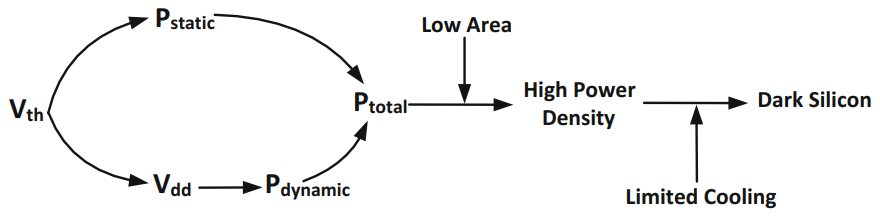
\includegraphics[width=0.7\textwidth]{Dark silicon problem diagram.png}
		\label{Dark silicon problem diagram}
	\end{figure}

	Observing Figure~\ref{Dark silicon problem diagram}, the flowchart of dark silicon can be followed. Condensing power into a smaller area without equivalent advancements in cooling technology results in silicon that can't be safely powered. Dark silicon represents a significant challenge in CPU design, as it broadens the range of considerations that need to be addressed to get maximum performance out of a chip.

\section{Scope}
	\underline{Original Scope:}
	\begin{center}
		\begin{tabular}{|c|c|}
			\hline
			In Scope & Out of Scope\\
			\hline
			Digital Design & Material Design\\
			Task Scheduling Methodologies & Thermal Management\\
			Dynamic Frequency Scaling & Dynamic Voltage Scaling\\
			Memory Driven Computing & Reduced Area Design\\
			Heterogeneous Cores & \\
			\hline
		\end{tabular}
	\end{center}

	Originally, the scope for this project dismissed thermal management from the scope as irrelevant on an FPGA. On reflection, thermal management is a vital inclusion for any investigation of dark silicon methodology.
	
	\vspace{5mm}
	\noindent
	\underline{Revised Scope:}
	\begin{center}
		\begin{tabular}{|c|c|}
			\hline
			In Scope & Out of Scope\\
			\hline
			Digital Design & Material Design\\
			Task Scheduling Methodologies & Dynamic Voltage Scaling\\
			Dynamic Frequency Scaling & Reduced Area Design\\
			Memory Driven Computing & \\
			Heterogeneous Cores & \\
			Thermal Management & \\
			\hline
		\end{tabular}
	\end{center}

	The scope for this project is slightly eclectic. This is a necessity driven by the broad, ranging research space of dark silicon. Solutions to the dark silicon issue are being developed by material scientists, using 3D architectures, photonic interconnects or diamond as a semiconductor instead of silicon. Whilst fascinating, these are all out of scope for a computer and electrical engineering thesis.
	
	Hardware oriented solutions tend to come in the forms of Dynamic Voltage and Frequency Scaling. In scope for this is Dynamic Frequency Scaling (DFS), however dynamic voltage scaling (DVS) is out of scope as it is difficult to implement on an FPGA. Additionally, the hardware oriented approached of heterogeneous cores and memory driven computing are in scope.
	
	Finally, task scheduling methodologies are in scope as resource allocation at an OS level is relevant to optimising CPU utilisation for dark silicon parameters.



	\leavevmode\thispagestyle{empty}\newpage
	\leavevmode\thispagestyle{empty}\newpage

	\chapter{Background Theory}
		
	\section{Dark Silicon}
		\subsection{Obituary for Moore’s Law and Dennard Scaling}
			The origin of Moore's Law stems from a paper released in 1965, titled \textit{Cramming more components onto integrated circuits}. In this paper, Moore predicted the number of transistors in an integrated circuit would double every 18-24 months \cite{BookOfMoore}. This relationship was representative of trends in computer development until round the mid 2005. Figure~\ref{SRAMGraph} shows trends on the spacing of components on chips, and as can be seen the trends slows down around the 2005-2010 mark.	Around the same time, Dennardian Scaling was experiencing a similar downfall.
			
			In 1974, Robert H. Dennard et al. released a paper titled \textit{Design of ion-implanted MOSFET's with very small physical dimensions}, in which he observed the relationship between transistor size, frequency, capacitance and and operating voltage $V_{DD}$. He found that for fixed power and area budgets, an exponential increase the maximum number of transistors that will fit into the area results in a linear increase in maximum operating frequency \cite{SmallDimensionMosfets}. This can be seen in Figure~\ref{DennardianScalingTable},and is termed Dennardian Scaling. A 33 year review of Dennard et al. in 2007 found that the assumptions that underpinned Dennardian scaling were inadequate. For example, it was assumed that MOSFET channel doping concentrations would continually increase, producing shorter channels with each generations. In reality, it was found that as the concentration of channel doping increases, impurity scattering caused the carrier performance and mobility to degrade. A number of Dennards assumptions failed, and this resulted in Post-Dennardian Scaling, which can also be seen in Figure~\ref{DennardianScalingTable}, where the operating voltage has ceased to decreased with transistor size and so the power requirements of new generating are exponentially increasing. Conversely, we see on chip utilisation for a fixed power budget decreases exponentially.\cite{ReviewOfDennard}.
			

			\begin{figure}

				\begin{center}
					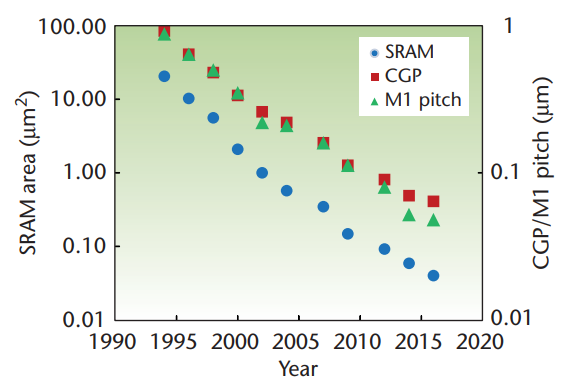
\includegraphics[width=0.5\textwidth]{SRAM CGP and M1 Pitch Graph.png}
				
				\caption{Historical data from the last 20 years of chip development \cite{TheEndOfMooreTheis}.}
				\end{center}
				\label{SRAMGraph}
			\end{figure}
		
		
			\begin{figure}
				
				\begin{center}
					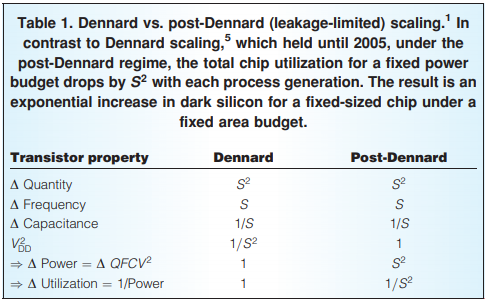
\includegraphics[width=0.5\textwidth]{Dennardian scaling table.png}
					
					\caption{Ratios in Dennardian and Post-Dennardian Scaling. \cite{TheEndOfMooreTheis}.}
				\end{center}
				\label{DennardianScalingTable}
			\end{figure}
			
		\subsection{The minimum energy for computing}
		
			In the 20th century, Charles H. Bennet et al. proved that for any irreversible computation there is a minimum amount of switching energy required, equivalent to $k|{B}T\ln{2}$, where k is the Boltzmann constant, and T is the temperature. At room temperature this is approximately $10^{-21}$J, or 1 zeptojoule. This limit is called the Shannon-von Nuemann-Landauer limit and it is descriptive of switching elements' physical properties, specifically that the lower power limit for their function is very low. The relevance of this is thus: a driving factor in dark silicon is that as transistor size reduces, transistor power usage still reduces. Though the new trend of increating power density is linked to decrease in transistor size, transistors are not the limiting factor. The limiting factor is that transistors are no longer the primary source of energy consumption \cite{MinEnergyInComputing}.
			
			The primary source of energy consumption in embedded electronics is electrical capacitances. In integrated circuits, the most common forms of capacitance are wire interconnects. Short interconnects are modelled as capacitive lumps in the circuit, while medium length interconnects are modelled as lossy RC transmission lines and long interconnects are modelled as lossy RLC transmission lines. As transistor size scales down, these interconnects are becoming the dominant limitation for clock frequency, power utilisation and transmission delay in-circuit.
			
			In contemporary microprocessors in the 22-65nm range, the total energy consumptions attributed to transistors makes up only ~20-30\% of the total energy budget. This percentage is expected to decrease as transistor size decreases \cite{MinEnergyInComputing, Interconnects}. 
		
		
		
		
		\subsection{The Four Horsemen of Dark Silicon}
			As we move into an era of CPU design defined by Post-Dennardian Scaling, we must address the exponential decrease in chip area utilisation. This decrease has a significant effect on multicore scaling, as fitting more cores onto chip requires those cores to be under-clocked, underpowered, or not powered at all. In an article titles \textit{The Four Horsemen of Dark Silicon}, Michael B. Taylor categorised the primary methods for resolving the dark silicon problem. He refers to them as the "4 Horsemen", and ordered from most to least relevant they are:
			
			\begin{itemize}
				\item \textbf{The Specialised Horseman} - Heterogeneous core design.
				\item \textbf{The Dim Horseman} - Under-clocked or underpowered cores. 
				\item \textbf{The Shrinking Horseman} - Reduced area core design.
				\item \textbf{The Deus Ex Machina Horseman} - Material science advancements.
			\end{itemize}
		
			\subsubsection{The Specialised Horseman}
				A typical ASIC circuit is usually 100 to 1000x faster than a general processing unit, as well as 157 to 707x more energy efficient for a given task \cite{InefficiencyInGeneralPurposeChips}. While achieving these levels or performance and power efficiency is unlikely in a general processing unit, attempting to imbue a softcore with these properties would, if successful, produce a core that performs tasks faster, with a lower power budget, at the cost of an expanded area requirement. Dark silicon leaves us with a surplus of space and a deficit of power, making design choices that trade expanded circuitry for minimized power budgets ideal \cite{DarkSideOfSilicon, TheFourHorsemen}.
				
			\subsubsection{The Dim Horseman}
				A cousin of dark silicon is dim silicon. Dim silicon refers to under-clocked or underpowered sections of the chip. By reducing the voltage or frequency, the power budget can be met. For example, Figure~\ref{DimSilicon} shows a an example dim silicon implementation, with an increase in core numbers but no increase in clock frequency. Dynamic Voltage and Frequency Scaling are dim silicon methodologies and DFS is of interest to this project, as it can be implemented in an FPGA using controlled prescalers.
				
				Computation sprinting is a form of DFS where the chip spends most of its time in an under-clocked state, and spends short bursts or "sprints" in at a higher clock rate that produces excessive heat on chip. Once the heat reaches a safety-limit, the chip is returned to a low clock rate, and the heat is allowed to dissipate. This allows for a balance while managing energy and thermal considerations. This method can be implemented in a multicore system \cite{ComputationalSprinting}.
				
				Underpowered silicon involves running sections of the chip at a lower voltage than the transistors are rated for, the power budget can be reduced in exchange for an increased risk of metastability. This is called Near Threshold Voltage processing. This method is out of scope for this project, for the same reason as DVS \cite{DVS}.
				
				\begin{figure}
					\centering
					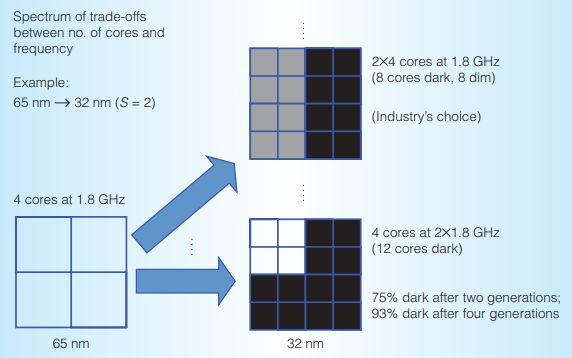
\includegraphics[width=0.7\textwidth]{DimSilicon.png}
					\caption{text}
					\label{DimSilicon}
				\end{figure}
			
			\subsubsection{The Shrinking Horseman and the Deus Ex Machina Horseman}
				The Shrinking Horseman refers to what I have termed reduced area design. The design methodology is in the label: shrink the size of CPU's and use smaller die. By simply removing the dark silicon from the chip, the problem is neatly sidestepped. This solution is not in the scope of this project.
				
				The Deus Ex Machina Horseman refers to the aforementioned advances in material design. Again, the method is in the label: a god-out-of-the-machine event might remove the constraints of dark silicon by increasing the allowable power budget a CPU can handle, or by decreasing the power budget required for modern computing. Already scientists are experimenting with different semiconductor substrates, 3 dimensional chip designs and photonic interconnects, each of which could resolve the dark silicon problem. Photonic interconnects in particular could be extremely efficient as a solution to the problem of lossy RC and RLC interconnects. Nonetheless, this is the realm of material scientists and is outside of the scope of this project \cite{TheFourHorsemen}.
			
		\subsection{Memory Driven Computing}
			Memory Driven Computing is an attempt to deal with the power constraints caused by interconnects. In a standard computers, memory is stored in multiple units at varying distances from the computing unit. The closer the memory units is to the CPU, the less memory it can hold. This varied memory model is used because the memory closer to the CPU tends to be more expensive per bit, in a relationship described in Figure~\ref{StorageDeviceHierarchy}.
			
			\begin{figure}
				\centering
				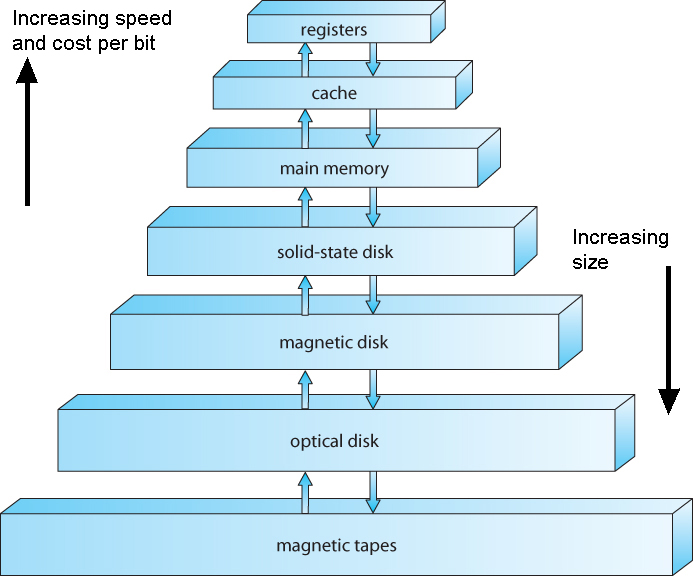
\includegraphics[width=0.5\textwidth]{StorageDeviceHierarchy.jpg}
				\caption{Computer Memory System Model \cite{CPUScheduling}}
				\label{StorageDeviceHierarchy}
			\end{figure}
		
			A similar principle at chip level is used in placing cache memory: it is often located on one section of the chip, with the core or cores elsewhere. This can lead to large interconnects required to join the memory with the core or cores. Memory Driven Computing seeks to distribute cache memory around the chip, specifically to be close to the core or cores, reducing the number of large interconnects on the chip required to move memory around \cite{EndOfMooresLawWilliams}. 
		
		\subsection{The Dark Side of Silicon}
			In 2017, Rahmani et al. released a book title \textit{The Dark Side of Silicon}, spanning a collection of works in the dark silicon research space. This book is a fountain of information for dark silicon design methodologies, and outlines a combined hetergeneous methodology and memory driven computing methodology that inspiration is drawn from.\\
			The SiLago methodology was developed to remedy the following issues in CPU design:
			\begin{itemize}
				\item Most design focuses on cores, ignoring memory and inteconnects
				\item Software layer abstractions often employ naive resource allocations, which results in runtime inefficiencies.
				\item A absence of dynamic customization at runtime means that non-deterministic concurrency and communications patterns produce power usage and parallelism inefficiencies.
				\item Over-customisation is prohibitive due to large engineering costs.
			\end{itemize}
			The SiLago methodology answers these problems by implementing a distributed memory architecture. This directly combats losses from interconnects and has been shown to significantly reduce power and energy expenditure on chip when properly implemented \cite{SiLagoSolution}. Similar methodologies have shown that arbitrarily placing memory through the chip significantly reduced the power losses from on-chip interconnects \cite{DynamicDirectories}.
	
	\section{Task Scheduling}
		
		\subsection{Algorithms}
			The aim when scheduling for CPU's is to maximum resource allocation usually by pausing a program while it waits for a I/O or system call commands to return. Scheduling attempts to maximise CPU utilisiation, data throughput, task turnaround time, task waiting time (time spent waiting on I/O or systems calls, etc.) and task response time (how long a task waits in the queue before reaching the CPU).
			
			Priority scheduling approaches this by assigning tasks different priorities. This ensures that the most important tasks aren't blocked by less important tasks, though it can result in less important tasks being blocked for extended periods. A solution to this is a Multilevel Feedback Queue, which uses multiple queues to designate tasks that have been waiting or running for different periods of time. It ensures that priority is given to the most relevant tasks, whilst also preventing less important tasks from being ignored \cite{CPUScheduling}.
		
		\subsection{Variation Aware Core Selection}
		 	In conjunction with heterogeneous core implementation, there is the scheduling methodology called Variation Aware Core Selection. This methodology utilises the heterogeneous nature of an implementation to schedule tasks to the core best suited for their workload. This fusion between good hardware design is an example of the way to get the best performance out of chips by utilising an ASIC like implementation. Without the variation aware resource allocation, the heterogeneous implementation would be wasted. \cite{HeterogenousCoreDesign}.
			
		
	
	\section{Thermal Considerations}
		\subsection{Thermal Hotspots}
			Heat distribution on chip is non-uniform and non-trivial. Their are a number of temperature gradient that exist across the chip, typically described by a number of hotspots on the chip. Hotspots present an issue wherein a localised section of a chip risks damage. The distribution varies with workloads, and differs between die due to physical variations (e.g. thickness of substrate), and in a multicore system this distribution is an product of the interactive heat dissipation from the different cores. As shown in Figure ~\ref{fig:DieHotspots}, hotspots tend to arise in the regions of the die allocated for cores, though they arise in a variety of function units, such as I-cache, D-cache or floating point units. The tendency of a region to become a hotspot is workload dependent.  . 
			
			\begin{figure}[h]
				\centering
				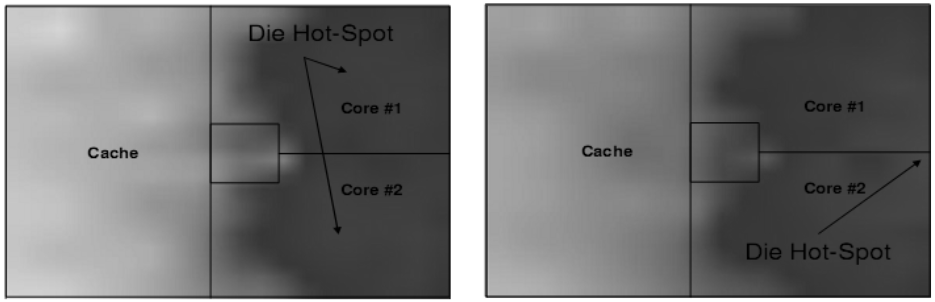
\includegraphics[width=0.7\textwidth]{DieHotspots.png}
				\caption{Heatmaps of local hotspots on a multicore die under different workloads \cite*{HotspotsInDie}}
				\label{fig:DieHotspots}
			\end{figure}
		
			A hotspot acts a pole for temperature. The heat dissipation around this pole can be modelled using the formula 
			\begin{equation}
				T(x,t) = \frac{Q}{2 \pi \lambda x} \left[ 1-\frac{2}{\sqrt{\pi}} \sum_{n=0}^{\infty} (-1)^n \frac{r^{2n+1}}{\prod_{n=1}^{n}n(2n+1)}) \right]
			\end{equation}
			which in steady state, as $t \to \infty$, becomes equivalent to 
			\begin{equation}
				T(x) = \frac{Q}{2 \pi \lambda x}
			\end{equation}
			As the dimensions of the die decrease, if a heat-naive layout is maintained, the dissipation areas around the hotspots overlap, putting sectors between hotspots at risk of degradation. Layout that herd hotspots into each other proximity create temperature bottlenecks for temperature that reduces the quality of temperature dissipation across the chip for all hotspots. The solution to combat this is the distribute likely hotspots across the chip, giving them a larger area around themselves to dissipate heat.
			
			In particular, several software methods utilise this approach by apportioning workloads to different function units in the die. These methods reduced the hotspot temperatures and the average temperature across the die \cite*{HotspotsInDie}.

		\subsection{Dynamic Thermal Management and Hotspot Management}
			Dynamic Thermal Management (DMT) is emerging as an alternative to traditional solid state thermal management. The goals is to make cooling routines adaptive to the circumstances to make them more effective. Particularly of interest here is DTM with regards to hotspot management. While hotspot remediation is still progressing as a field, several examples of it are cropping up and they present opportunities in the land of dark silicon. For example, Bar-Cohen et al. experimented with using Mini-Contact Enhanced Thermo-Electric Coolers, In-Plane Silicon Microcoolers, Si/SiGe Superlattice Microcoolers and Microgap coolers, and found they could reduce hotspot temperatures by as much as 17$^{o}$C, in the context of a hotspot 37$^{o}$ hotters than surrounding silicon \cite{Bar-CohenAvram2012Tmoo}.
			

		\subsection{Thermal Aware Design}
			Thermal aware design is a CPU implementation method that takes cooling procedures into account. Fully realised thermal aware design involves tailoring thermal management of the CPU as well, which is out of the scope of this thesis. A key consideration is that thermal aware designs do not necessarily translate well between different chips. So, thermal aware considerations in this project come with the assumption that these design will be possible in the future. The practical thermal management is out of the scope of this project, but utilising thermal management in the context of hotspot management fits neatly into the dark silicon ballpark. Appropriate thermal aware design can produce considerable improvements in efficiency over non-thermal aware design methodologies, so it is worth designing chips with the capacity to employ thermal aware methodologies in the future \cite{ThermalAwareDesign, ThermalSafePower}.
	
	\section{RISC-V}
		\subsection{The RISC-V ISA}
			The RISC-V ISA is a reduced instruction set architecture. It is useful in an open source context as it comes in multiple bit-lengths and is entirely modular. The base instruction set contains standard logic flow control functions, standard IO and addition and subtraction. Additional modules add functionality for multiplication and division, atomic functions, floating point operations, control status register implementation and more. The full outline can be found in \textit{The RISC-V Instruction Set Manual Volume I: Unprivileged ISA} \cite{riscvUnprivIsa, riscvPrivIsa}.
		\subsection{RISC-V Cores}
			Different cores implement different levels of the RISC-V ISA. For the sake of later discussion, the following warrant mention:
			\begin{itemize}
				\item \textbf{RISC-V Processing UNIT (RPU)} implements the base instruction set and the control status register instruction set in 32-bit architecture.
				\item \textbf{InstantSOC} implements the base instruction set and the multiplication instruction set in 32-bit architecture.
				\item \textbf{VexRiscv} implements the base instruction set, the multiplication set and the control and status register instruction set in 32-bit architectures \cite{riscvCores}.
			\end{itemize}
			
		
	
	
	\leavevmode\thispagestyle{empty}\newpage
	
	\leavevmode\thispagestyle{empty}\newpage
	
	\chapter{Method}
	\section{The Initial Plan}
	\subsection{Overview}
		The initial plan was to determine an adequate RISC-V softcore for the mixed hardware and software modifications that were intended to be completed. The chosen core was RPU. Once selected, this core was to be uploaded onto an FPGA, and brought to an operational level with an OS running on it. At this stage, a series of test algorithms would be run with metrics collected in order to establish a baseline of performance. This baseline was to be used to contrast against the improved softcore implementations. First, several dark silicon methodologies were to be implemented individually, then successful methodologies were to be merged into a final working model. This final working model would be used to produce the data for the final A visual outline of this is shown in Figure~\ref{ThesisFlowchart}. 
		
		\begin{figure}
			\centering
			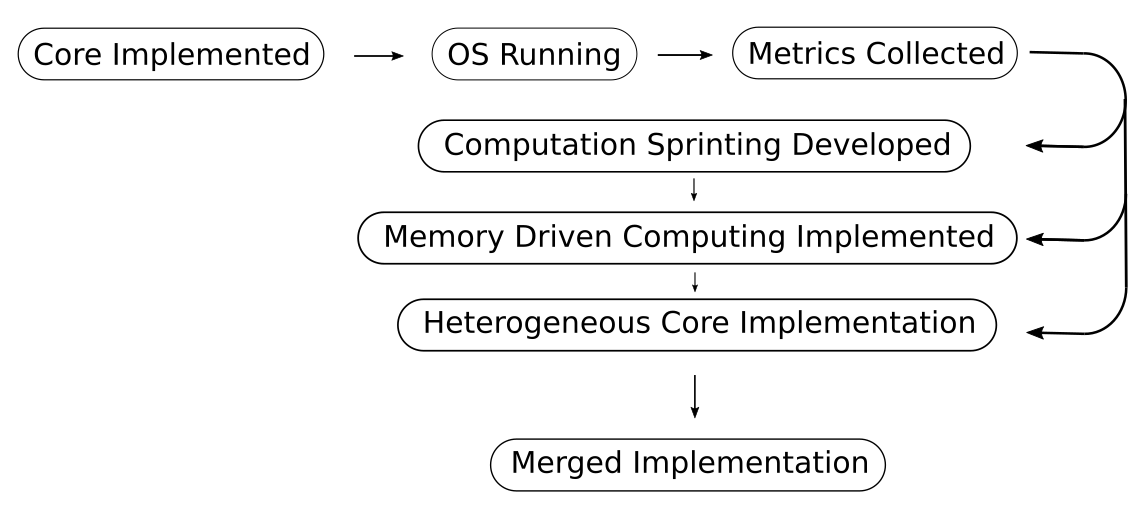
\includegraphics[width=0.8\textwidth]{ThesisMethodFlowchart.png}
			\caption{Flowchart of Thesis implementation}
			\label{ThesisFlowchart}
		\end{figure}

	
	\subsection{Software Packages Used}
		\textbf{VMWare} - Used to handle the virtual machine\\
		\textbf{Ubuntu 20.4} - Used as the OS for RISC-V compilation.\\
		\textbf{RISC-V GNU Toolchain} - To compile RISC-V code.\\
		\textbf{Python} - For scripting and to transpile RISC-V ASM into 32 bit machine code for RPU. \\
		\textbf{Vivado} - For programming the FPGA boards. 
	
	\subsection{Hardware Packages Used}
		\textbf{Computer} - This project required a Vivado setup and a virtual machine to handle the RISC-V installation.\\
		\textbf{Rice University WARP2} - Initial FPGA board intended for this project, which was discarded partway through the project.]\\
		\textbf{Nexys 4 DDR} - An FPGA board on which a core was implemented.
	
	\subsection{Project Plan}
		Each dark silicon methodology needed to be developed and tested in a set time frame in order to test combinations of methodologies at the end of the process. The following schedule marked milestones with hardware, with firmware development being performed in tandem. The software modifications were intended to be performed mostly by cycling through already present methodologies on the linux system, with minimal tweaks being performed. Once all of the different methodologies had been implemented and tested, final tweaks would be performed on the optimal system, from which the final results would be derived.
		\subsubsection{Project Schedule and Timeline}
		
		\begin{center}
		\begin{tabular}{ c|c }
		August 2019 & RISC-V softcore implemented on FPGA, with running Linux Kernel.\\
		September 2019 & Control and sensitivity testing of metrics \\ & Control data collected from Linux.\\
		October 2019 & Begin optimisation for memory driven computing.\\
		November 2019 & Testing basic datasets for memory driven and computational sprinting.\\
		December 2019 & Begin work on heterogeneous cores.\\
		February 2020 & Test basic datasets with heterogeneous cores and computational sprinting.\\
		March 2020 & Test basic datasets on heterogeneous cores with memory driven computing.\\
		April 2020 & Implement project as general computer with TRL of 6.\\
		May 2020 & Poster and demonstration prepared.\\
		June 2020 & Thesis completed and submitted.\\
		\end{tabular}
		\end{center}
	
	\subsection{Technology Readiness Level}
		The goal is to achieve TLR 6 on the following scale.
		\begin{itemize}
			\item \textbf{TRL 1} – Task scheduler optimised, metrics display improvement over baseline testing.
			\item \textbf{TRL 2} – Task scheduler displaying clear trends of optimizations and can process basic workloads.
			\item \textbf{TRL 3} – Task scheduler can be used to process moderately complex workloads.
			\item \textbf{TRL 4} – Task scheduler running Linux with evidence of optimisation
			\item \textbf{TRL 5} – Task scheduler, can be used for general purpose computing under controlled circumstance and settings.
			\item \textbf{TRL 6} – Task scheduler optimal allocating resources over a variety of robust workloads.  Capable to be used as a low function PC.
		\end{itemize}



	\subsection{Algorithm Schemes}	
		The initial plan was to implement a round robin scheduler, a priority queue scheduler and a hybridised scheduler, to produce diversity of data. The testing was to consist first of a Fast Fourier Transform (FFT) during the proof of concept stage, the results of which would be used as a heuristic to judge the quality of iterative improvements. After modifications had been made to the algorithms and the core, the goal was to use Dhrystone, Geekbench and CoreMark to test the quality of the different dark silicon methodologies in use.\\
		While some of these programs have received criticism for the quality and usefulness as benchmarks, for the use of a before and after dataset, they are adequate. Scheduling algorithms that use Variation-Aware Core Selection and Scheduling will also be an important methodology for reducing the amount of naïve scheduling caused by abstraction away from the hardware layer.
	
	\subsection{Performance Metrics}
		The control metrics will be:
		\begin{itemize}
			\item Test algorithm runtime
			\item Power and energy requirements
			\item Quality of resource allocation
			\item Area of chip used.
		\end{itemize}
	
\section{Implementation Designs}
	\subsection{Computational Sprinting}
		The computational sprinting design will vary a prescaler at set intervals. The setup for this is displayed in Figure~\ref{CompSprint}.
	
	\begin{figure}
		\centering
		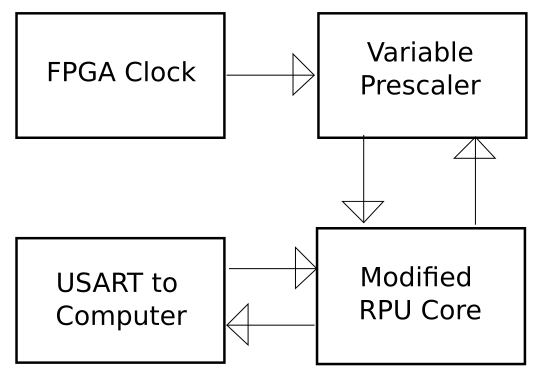
\includegraphics[width=0.5\textwidth]{CompSprint.png}
		\caption{Computation Sprinting Implementation}
		\label{CompSprint}
	\end{figure}
	
	\subsubsection{Sprint Switching}
		A subsection of the computation sprinting design would be to consider a sprint switching design. This methodology considers the tendency of hotspots to build around cores. Implementing hotspot management techniques would be ideal for this project, but this method  mostly relies on switching which core is sprinting at any given point in time, so that the total energy in the system stays consistent and hotspots don't overlap.
	\begin{figure}
		\centering
		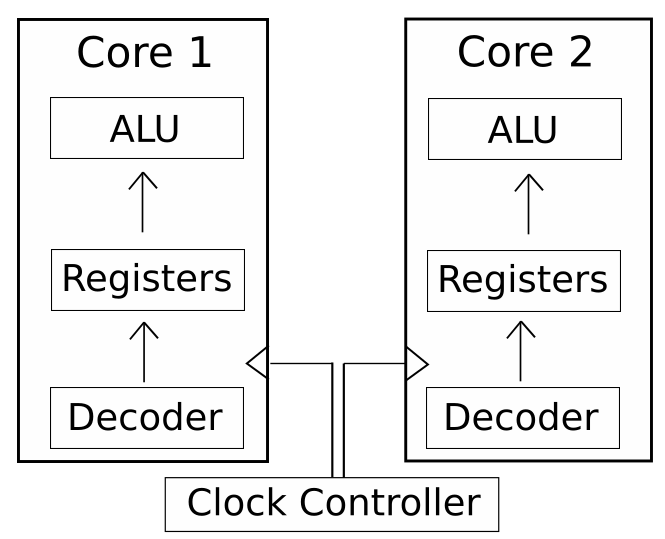
\includegraphics[width=0.5\textwidth]{Switched Sprinting.png}
		\caption{Sprint Switching Implementation}
		\label{Sprint Switching Implementation}
	\end{figure}
	
	\subsubsection{Single Threading Switching}
		A single threaded variant on sprint switching would involve connecting the registers of multiple cores so a core can be sprinted,and when that core becomes too hot, the register values are pushed over to another core, which is then sprinted. The precise method of joining cores would need to be designed to reduce interconnect size. 
	\begin{figure}
		\centering
		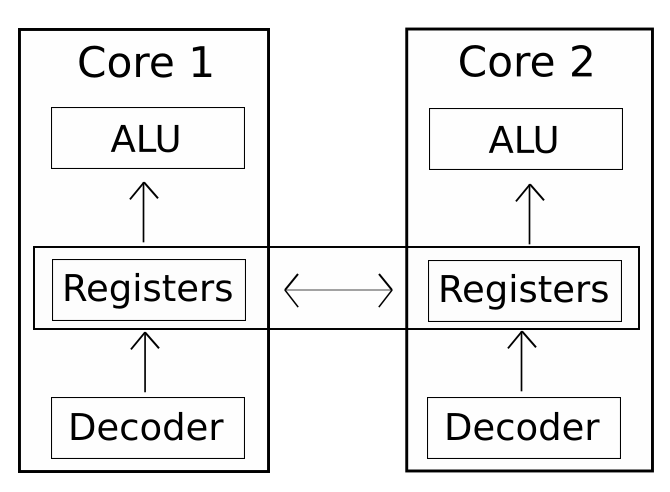
\includegraphics[width=0.5\textwidth]{SingleSwitching.png}
		\caption{Single Threaded Switching Implementation}
		\label{Single Threaded Switching}
	\end{figure}

	\subsection{Memory Driven Computing}
	The memory driven computing implementation would involve placing memory around and between the different cores, as displayed in Figure~\ref{MemDriven}.
	\begin{figure}
		\centering
		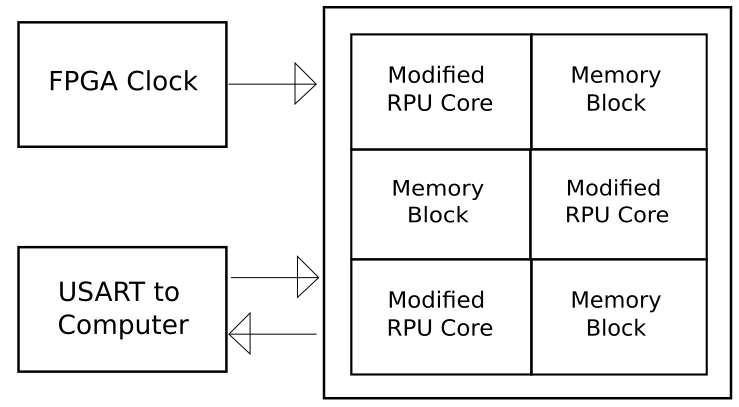
\includegraphics[width=0.5\textwidth]{MemDriven.png}
		\caption{Memory Driven Implementation}
		\label{MemDriven}
	\end{figure}

	\subsection{Heterogeneous Cores}
	The heterogeneous core implementation would involve tying multiple cores together with the main controlling core linking them together as shown in Figure~\ref{HetCores}.
	\begin{figure}
		\centering
		\includegraphics[width=0.5\textwidth]{HetCores.png}
		\caption{Heterogeneous Implementation}
		\label{HetCores}
	\end{figure}

	\subsubsection{Reduced Frequency Cores}
	A variant on the heterogeneous core design methodology would be to use cores that vary by their critical path length. Reducing the maximum clocking frequency of a core reduces the maximum critical path. Using smaller transistors, and taking advantage of the increase area budgets of dark silicon chips, an increased critical path could allow the number of pipelining stages to be reduced. If this can be done in a way that doesn't sacrifice performance, this could be a valuable way to exploit the loosened area constraints. This can also allow cores to be chosen based on how conducive they are to different levels of pipelining.
	\begin{figure}
		\centering
		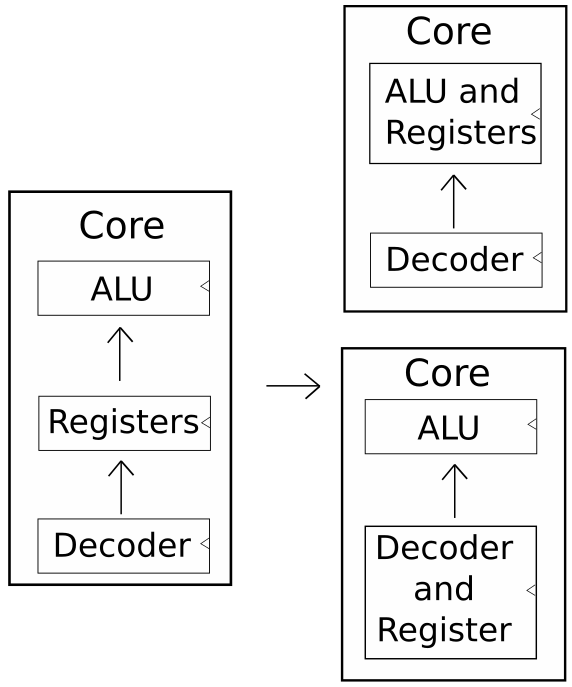
\includegraphics[width=0.5\textwidth]{ReducedFrequencyCores.png}
		\caption{Reduced Frequency Implementation}
		\label{ReducedFreqCores}
	\end{figure}



	

	
	\chapter{Results}
	\section{The Outcome}
	Throughout this project, the author has:
	\begin{itemize}
		\item Developed extensive knowledge of the world of RISC-V softcores.
		\item Learnt the finer points of the RISC-V ISA.
		\item Developed a basic RISC-V ASM to Machine code transpiler in python.
		\item Discovered a variety of ways to not implement an OS on a RISC-V system.
	\end{itemize}

	Unfortunately, aside from implementing the CPU on an FPGA, no other results were produced for this project.
	
\section{What Went Wrong}
	This thesis was supposed to generate a working model of a soft core processor running an OS. This has not come to pass, and so it is important to evaluate the combination of forced and unforced errors that accumulated during this project as well as events outside of the authors control, to contextualise the timeline.
		
	\subsection{The Scope}
		Setting hardware modification as the goal of this project may have been a mistake. While it is possible to get an OS running on a RISC-V machine with relative ease, this is only for set machines, none of which existed in a language the author was familiar with. A Venn diagram of ease to modify on a hardware level and ease to implement an OS on the softcore may overlap, but they do no overlap in the realm of VHDL. The broad scope of the project meant that research focus had to cast a wide net to find methods to cover a multitude of factors and approaches, and so the specific implementation was glossed over in the early phases, based on a satisfaction that OS implementation was a known possibility.
		
	\subsection{Assumptions}
		Two reasonable assumptions to make are that modifying a softcore CPU is a complicated process, and that implementing an OS on a softcore CPU could be a complicated process. The flawed assumption made in this project was that uploading an OS onto a softcore CPU would be relatively easy, and worthwhile if it allowed the use of an easier to modify softcore CPU. RPU had no implemented OS at the beginning of this project, but was easier to use and understand that other VHDL cores that were considered. Uploading an OS onto the RPU core turned out to be a more difficult experience than had been initially expected, however additional disruptions that were unrelated to the projects scope make it hard to say whether this would have had as much of a negative effect on the project had there been more time to approach the problem.
		
		It was also assumed that picking a core in a known language would be preferable to picking a core in an unknown language. While this is typically the case, a new conclusion has been drawn that if the task is more complicated than the new language is, learning a new language should not be a constraint in tool selection.
	
	\subsection{Key Events}
		A trio of large events impacted time management and productivity during this project. The first was a medical event which negatively impacted the first semester, the second was house move that impacted the end of year holiday period and the final event was the global pandemic of COVID-19 which impacted the second semester.
		
	\subsection{Forced Errors}
		A large drawback in this project was the unexpected complexity of setting up the environment. The initial hardware I was given required a specialised but depreciated environment, which took a considerable amount of time to set up first on Windows 10, and then again on a Windows 7 Virtual Machine, only to discover that the full installation would take a debilitating time to set up. My supervisor suggested a moved to an alternate piece of hardware, which resolved the issues, but by this stage several weeks were already casualties to fruitless debugging and forum based research. The new hardware had an easy environment to set up and at the end of the semester the project had a working environment, but behind schedule on additional research and implementation.\\
		
		
	\subsection{Unforced Errors}
		The holiday period was extremely dense on work and preparations for moving houses, so an assumption was made that the thesis work could be caught up with during the second semester. The unforced error here was not pushing through additional work during the holidays. While it was impossible to predict the COVID-19 pandemic, further work done during this period would have offset issues faced a later junctures. It also would have helped to discover dead ends earlier in the project, allowing for appropriate replanning.\\
		Beginning the second semester, the plan was to catch up on additional research and spend the first several weeks streamlining the rest of the semester so a majority of the semester could be spent on thesis work, as would be required. Some progress was made in teasing out the workings of the RPU core, but a majority of work was put into preparing for the mid-late period of the semester.\\
		The other unforced error was the choice of RPU due to its low level nature and readiness for adaptation. Choosing a harder to modify, but easy to set up processor would have been preferable, as the difficulty of implementing an OS on RPU ultimately was a massive detraction from the project.
		
	\subsection{Sunk Cost Fallacy}
		During this project there were many dead ends and junctures where a choice had to be made to continue with an approach that wasn't working or abandoning lost time and finding a new approach. During the first half of the project many dead ends were hit and methods abandoned in the hope of greener pastures that never appeared. During the second half of the project, an attempt was made to stick to a single approach, based on the seemingly reasonable assumption that that method would pay off.
	

	
\section{A Revised Approach}
	With the 20/20 vision of hindsight, a different approach should be taken to this project. Preferable, more specialised hardware should be sourced, as the RISC-V space tends to lend itself most to specific hardware, in part because this hardware helps to break the environment choice out from Vivado. Vivado is an excellent FPGA environment, but not necessarily the best environment for RISC-V development. Different cores should be considered, with less of a language based limitation. If hardware modification is the goal, the best approach to take on this project would be to start with a functioning OS with easy to modify scheduling software, such that the OS and the scheduling software are parameters in the data generation, but not complexity in the methodology. The hardware design itself presents a broad range of complexities.
	
	\subsection{Possible Hardware}
	\textbf{SiFive Board} - One of the more advanced RISC-V capable boards, these have a lot of support and a lot of pre-done implementations.
	\textbf{ArtyS7} - This board is used and support by many RISC-V projects. Uses the same Artix-7 FPGA chip as the Nexys 4 DDR.
	SiFive are involved in writing the RISC-V ISA specifications, and so their environment is specially made to work with RISC-V cores. The ArtyS7 uses the Vivado environment, but is an extremely popular board with RISC-V implementers, and so should be considered for ease of implementation.
	
	\subsection{Possible Cores}
	\textbf{VexRISC-V} - Initially dismissed because it is written in SpinalHDL, a Scala based HDL, this core seems very capable.\\
	\textbf{AndesCore} - Initially dismissed because it is written in verilog and listed as having no OS capabilities.
	
	\subsection{Revised Timeline}
	
	\subsection{TLR}
	Unchanged.
	
	\subsection{Zephyr - an OS alternative}
	Zephyr is not listen on the RISC-V site, but is a viable OS for several RISC-V cores. This core is of particular interest as in mid-May, Domipheus, the author of RPU, implemented this OS onto RPU. Unfortunately he did not leave any guide on how to replicate this, and on request for further information, revealed that the OS needed to be partially rewritten due to the fact that RPU lacked the multiplication extension. 
	
	\subsection{Key Approach}
	Instead of trying to build upwards from a basic core up to an core running a kernel, it is advisable to start with an already working system. There is a lot of complexity to work out in this approach but it means that single core methodologies could be easily implemented and there is model to compare multicore adaptations against.
	
	\subsection{Refined Scope}
	Placeholder for a refined scope for the project. Best scope would be in 2 flavours: split into a multicore approach that focusses on priority task scheduler, and a single core approach that varies the task scheduling and implements computational sprinting. 
		
	
	\chapter{Conclusion}
	Placeholder.
	
	\appendix
	\chapter{Appendix}
%	\input{chapters/appendix}

%	\nocite{*}
	\printbibliography
\end{document}
